\documentclass[conference]{IEEEtran}
\IEEEoverridecommandlockouts
\usepackage{amsmath,amssymb}
\usepackage{algorithm}
\usepackage{algpseudocode}
\usepackage{booktabs}
\usepackage{array}
\usepackage{xcolor}
\usepackage{tikz}
\usetikzlibrary{arrows.meta,positioning,fit}
\usepackage[hidelinks]{hyperref}

\begin{document}
\renewcommand{\arraystretch}{0.85}
\setlength{\tabcolsep}{4pt}
\setlength{\textfloatsep}{4pt plus 1pt minus 1pt}
\setlength{\dblfloatsep}{4pt plus 1pt minus 1pt}
\setlength{\floatsep}{4pt plus 1pt minus 1pt}
\setlength{\dbltextfloatsep}{4pt plus 1pt minus 1pt}

\title{SAGE (Semantic Analysis and Generation Engine): A Cross-Source Reasoning Engine over Heterogeneous Knowledgebases}

\author{
\IEEEauthorblockN{Srujan Zanjal}
\IEEEauthorblockA{
Computer Science and Engineering\\
St. Vincent Pallotti College\\of Engineering and Technology\\
Nagpur, Maharashtra, India\\
zanjalsrujan94@gmail.com
}
\and
\IEEEauthorblockN{Rimanshu Sonule}
\IEEEauthorblockA{
Computer Science and Engineering\\
St. Vincent Pallotti College\\of Engineering and Technology\\
Nagpur, Maharashtra, India\\
rimanshusonule00@gmail.com
}
\and
\IEEEauthorblockN{Pratik Bhoyar}
\IEEEauthorblockA{
Computer Science and Engineering\\
St. Vincent Pallotti College\\of Engineering and Technology\\
Nagpur, Maharashtra, India\\
pratikbhoyar156@gmail.com
}
\and
\IEEEauthorblockN{Tanisha Shingne}
\IEEEauthorblockA{
Computer Science and Engineering\\
St. Vincent Pallotti College\\of Engineering and Technology\\
Nagpur, Maharashtra, India\\
tanishashingne04@gmail.com
}
\and
\IEEEauthorblockN{Prof. Ayaz Khan}
\IEEEauthorblockA{
Computer Science and Engineering\\
St. Vincent Pallotti College\\of Engineering and Technology\\
Nagpur, Maharashtra, India\\
ayazahmedkhan.ngp@gmail.com
}
\and
\IEEEauthorblockN{\phantom{Pratik Bhoyar}}
\IEEEauthorblockA{
\phantom{Computer Science and Engineering}\\
\phantom{St. Vincent Pallotti College}\\\phantom{of Engineering and Technology}\\
\phantom{Nagpur, Maharashtra, India}\\
\phantom{pratikbhoyar156@gmail.com}
}
}

\maketitle

\begin{abstract}
Most retrieval-augmented generation (RAG) systems are built and evaluated over a single, homogeneous corpus of text. Practical knowledge work seldom fits that assumption. A user investigating a topic may accumulate a project website, several PDFs, a recorded lecture, and a code repository, then expect to query all of them through one conversational interface. We present SAGE (Semantic Analysis and Generation Engine), a system that ingests four structurally different source types (crawled websites, PDF documents, YouTube video transcripts, and GitHub code repositories) through a shared ingest-chunk-embed-index contract, and answers questions over them with a single retrieval-reranking-generation pipeline. Three design decisions anchor the system. First, a deterministic, non-generative \emph{source-overview chunk} makes broad questions retrievable without a second LLM call. Second, a hybrid semantic-lexical reranking formula, paired with a \emph{diversity floor}, guarantees fair citation representation across multiple sources. Third, a confidence heuristic gates refusal in a citation-only Grounded Mode, as opposed to an always-answering exploratory mode. We validate the system through its test suite and an isolated, end-to-end evaluation harness that exercises the unmodified production code against three live-ingested sources over fourteen query executions. A concrete design defect, the silent starvation of one source's evidence in multi-source queries, surfaced during testing and is corrected by the diversity floor. SAGE contributes a checkable set of engineering decisions for grounded QA over heterogeneous, real-world knowledgebases; it introduces no new retrieval or generation model, and we document its limitations candidly.
\end{abstract}

\begin{IEEEkeywords}
retrieval-augmented generation, multi-source retrieval, question answering, reranking, chunking, confidence estimation
\end{IEEEkeywords}

\section{Introduction}

This paper addresses grounded question answering over a knowledgebase whose contents are structurally heterogeneous: web pages, documents, video transcripts, and source code coexist and must be queried together. A retrieval-augmented generation (RAG) pipeline conditions the language model's answer on passages retrieved from an external corpus \cite{lewis2020rag}. Published RAG systems are, with few exceptions, designed and measured against a single textual corpus of uniform structure. Real knowledgebases are rarely that clean: a query must be routed to whichever source actually holds the relevant evidence and return a citation naming where it originated, forcing extraction, chunking, retrieval, and citation to behave as one contract across source types that share almost nothing in their native structure. That contract, rather than any individual retrieval or generation model, is the engineering problem this paper takes on.

SAGE (Semantic Analysis and Generation Engine) is such a system. It ingests four source types, crawled multi-page websites, PDF documents, YouTube video transcripts, and GitHub code repositories, into a common vector index, and answers questions against one, several, or all of a user's sources through a single pipeline that performs semantic-lexical reranking, enforces per-source citation diversity on combined queries, gates its own confidence, and streams incremental answers with citations. It does not propose a new retrieval or generation model; three of its engineering decisions appear uncommon in this particular combination:

First, \textbf{deterministic source-overview chunks}: SAGE synthesizes one additional chunk per source, placed first, built purely from the source's own statistics and excerpts with no LLM call, so broad questions such as ``what is this about'' are retrievable despite overlapping poorly with any single content chunk. Second, \textbf{a reranking-plus-diversity-floor combination discovered as a bug fix}: ranking purely by blended score across a combined-source query can silently starve one source of any citation, so the remedy reserves each combined source's single best chunk before filling remaining slots by score. Third, \textbf{a confidence heuristic that gates refusal, not just a display badge}: SAGE computes a scalar confidence score from retrieval evidence alone and uses it, before generation, to decide whether Grounded Mode should answer or refuse with a clarifying question, with a narrower exemption for video sources.

Section~\ref{sec:related} situates SAGE against prior work. Section~\ref{sec:architecture} gives its architecture, Section~\ref{sec:ingestion} the four ingestion pipelines, Section~\ref{sec:overview} the source-overview mechanism, and Section~\ref{sec:retrieval} the reranking and diversity-floor formulas. Section~\ref{sec:confidence} covers confidence, answer modes, and interaction; Section~\ref{sec:validation} reports validation, evaluation, and limitations; Section~\ref{sec:conclusion} concludes.

\section{Related Work}
\label{sec:related}

\textbf{Dense retrieval and RAG.} Dense retrieval runs from DSSM \cite{huang2013dssm} to dual-encoder retrievers such as DPR \cite{karpukhin2020dpr}, the design SAGE's pipeline descends from. RAG \cite{lewis2020rag} introduced conditioning a generator on retrieved passages; Fusion-in-Decoder \cite{izacard2021fid} extended it by aggregating evidence over many passages jointly, close to SAGE's multi-chunk context window. The broader space is catalogued by Gao et al. \cite{gao2023ragsurvey}. SAGE encodes with a distilled SBERT-family bi-encoder \cite{reimers2019sbert}, a MiniLM checkpoint \cite{wang2020minilm,wang2020minilmv2} distributed as \texttt{all-MiniLM-L6-v2} \cite{minilm_modelcard}, trading accuracy for the latency an interactive product demands; on our evaluation set two newer small encoders brought no retrieval gain (Table~\ref{tab:embeddings}).

\textbf{Reranking, hybrid retrieval, and chunking.} Cross-encoders \cite{nogueira2019bert} and late-interaction models such as ColBERT \cite{khattab2020colbert} improve on bi-encoder retrieval by scoring pairs jointly, at added cost. SAGE instead blends its bi-encoder score with a lexical term-recall score, following CLEAR \cite{gao2020clear}, BM25 \cite{robertson2009bm25}, and Reciprocal Rank Fusion \cite{cormack2009rrf}, avoiding a second neural pass. Fixed-size chunking with overlap remains dominant, though studied directly for chunk-size sensitivity \cite{jimenoyepes2024chunking}, context-preserving ``late chunking'' \cite{gunther2024latechunking}, and strategy comparisons \cite{merola2025chunking}; SAGE applies a sentence-aware chunker to text and a separate band chunker to video (Section~\ref{sec:ingestion}).

\textbf{Modality-specific retrieval and confidence.} Video QA \cite{lei2018tvqa,zhang2024llovi}, retrieval-augmented code completion \cite{husain2019codesearchnet,zhang2023repocoder,wu2024repoformer}, and multi-document reading \cite{sachan2021multidoc} each address one modality; SAGE trains none, instead normalizing all four into one embedding space (Sections~\ref{sec:overview}--\ref{sec:retrieval}). Gating refusal on retrieval evidence rather than generator certainty follows selective prediction under distribution shift \cite{kamath2020selective}, limits on self-reported confidence \cite{kadavath2022knowwhattheyknow}, and persistent hallucination \cite{ji2023hallucination}; retrieval augmentation separately lowers hallucination \cite{shuster2021retrieval}. Consumer tools such as NotebookLM \cite{notebooklm2023} and frameworks such as LangChain \cite{langchain} and LlamaIndex \cite{llamaindex} address an adjacent problem; SAGE is neither, so direct comparison lies outside this paper's focus.

\section{System Architecture}
\label{sec:architecture}

\begin{figure}[t]
\centering
\resizebox{0.8\linewidth}{!}{%
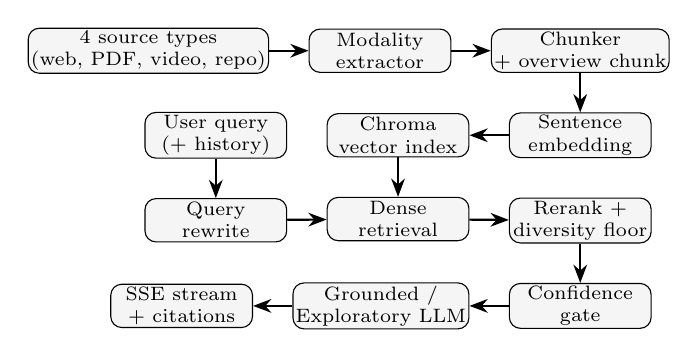
\begin{tikzpicture}[
  node distance=5mm and 5mm,
  box/.style={draw, rounded corners, align=center, minimum height=5.5mm, minimum width=18mm, inner sep=1pt, font=\scriptsize, fill=gray!8},
  arr/.style={-Stealth, thick}
]
\node[box] (src) {4 source types\\(web, PDF, video, repo)};
\node[box, right=of src] (extract) {Modality\\extractor};
\node[box, right=of extract] (chunk) {Chunker\\+ overview chunk};
\node[box, below=of chunk] (embed) {Sentence\\embedding};
\node[box, left=of embed] (index) {Chroma\\vector index};
\node[box, left=of index] (query) {User query\\(+ history)};
\node[box, below=of query] (rewrite) {Query\\rewrite};
\node[box, below=of index] (retrieve) {Dense\\retrieval};
\node[box, below=of embed] (rerank) {Rerank +\\diversity floor};
\node[box, below=of rerank, xshift=0mm] (conf) {Confidence\\gate};
\node[box, left=of conf] (gen) {Grounded /\\Exploratory LLM};
\node[box, left=of gen] (stream) {SSE stream\\+ citations};

\draw[arr] (src) -- (extract);
\draw[arr] (extract) -- (chunk);
\draw[arr] (chunk) -- (embed);
\draw[arr] (embed) -- (index);
\draw[arr] (query) -- (rewrite);
\draw[arr] (rewrite) -- (retrieve);
\draw[arr] (index.south) -- (retrieve.north);
\draw[arr] (retrieve) -- (rerank);
\draw[arr] (rerank) -- (conf);
\draw[arr] (conf) -- (gen);
\draw[arr] (gen) -- (stream);
\end{tikzpicture}}
\caption{SAGE end-to-end architecture: a shared ingest-chunk-embed-index contract feeds a single retrieve-rerank-gate-generate query pipeline.}
\label{fig:architecture}
\end{figure}

SAGE is a FastAPI backend with a React web client and a Chrome side-panel extension, backed by ChromaDB (vector store) and Supabase (relational store of record for sources, knowledgebases, and job status). Figure~\ref{fig:architecture} shows the two halves: an \emph{ingestion} half, where each source type is extracted by its own extractor into a common chunk representation, and a \emph{query} half, where every question passes through one retrieval, reranking, confidence, and generation pipeline.

A \emph{source} is one ingested website, PDF, video, or repository; sources are grouped into \emph{knowledgebases}, and a query can target a single source, an entire knowledgebase, or an explicit list of combined \texttt{source\_ids} spanning one or more knowledgebases. Every chunk, regardless of modality, carries a common metadata schema: a knowledgebase and source identifier, a source type, a chunk index, and a content-addressed chunk identifier computed as the truncated SHA-256 hash of the knowledgebase id, source id, chunk index, and chunk text, which makes re-ingestion of unchanged content naturally idempotent at the vector-store upsert layer.

\subsection{Persistence and Metadata}
Two stores back every source, kept in intentional sync rather than merged into one. ChromaDB holds only what retrieval needs: chunk text, embedding vector, and a flat metadata dictionary (Chroma rejects \texttt{None}-valued fields, so the upsert layer strips any unset field first). Supabase holds the relational structure the product needs but retrieval does not: knowledgebase and source records, titles, URLs, timestamps, and, for asynchronous source types, job status rows polled through \texttt{/jobs/\{job\_id\}}. A source's \texttt{chunk\_kind} field lets one shared context-assembly routine (Section~\ref{sec:retrieval}) special-case ordinary content chunks versus the source-overview chunk described next, without knowing which modality produced either. The background job tracker is a plain in-process dictionary with no persistence or expiry, a prototype simplification revisited in Section~\ref{sec:validation}.

Table~\ref{tab:endpoints} lists the system's REST surface.

\begin{table}[t]
\caption{SAGE API surface (\texttt{/api/v1} prefix)}
\label{tab:endpoints}
\centering
\scriptsize
\begin{tabular}{@{}l>{\raggedright\arraybackslash}p{3.1cm}>{\raggedright\arraybackslash}p{3.0cm}@{}}
\toprule
Method & Path & Purpose \\
\midrule
GET & \texttt{/health} & liveness check \\
POST & \texttt{/qa/ask}, \texttt{/qa/ask/stream} & sync QA / SSE streaming QA \\
POST & \texttt{/ingest/website}, \texttt{/ingest/pdf} & sync crawl / PDF upload \\
POST & \texttt{/ingest/video\allowbreak(-auto-transcribe)} & async transcript-API / Whisper fallback \\
POST & \texttt{/jobs/github-ingest} & async, only GitHub ingest path \\
GET & \texttt{/jobs/\{job\_id\}} & poll async job status \\
GET & \texttt{/sources(/grouped)}, \texttt{/sources/\{id\}/summary} & list sources / overview text \\
DELETE & \texttt{/sources/\{id\}} & delete source, its vectors \\
POST & \texttt{/sources/website/recrawl} & async re-crawl of a source \\
\bottomrule
\end{tabular}
\end{table}

Two details shape the rest of this paper. GitHub ingestion has no synchronous endpoint; it is always dispatched as a background job polled via \texttt{/jobs/\{job\_id\}}, unlike synchronous website and PDF ingestion. Video ingestion is exposed as two independent, explicitly user-triggered endpoints rather than one endpoint with an automatic fallback: \texttt{/ingest/video} attempts the transcript API and fails distinguishably if none exists, and the client separately offers a ``transcribe automatically'' action calling \texttt{/ingest/video-auto-transcribe}, with no server-side chaining between the two.

\section{Multi-Source Ingestion}
\label{sec:ingestion}

Each modality has its own extractor, but every extractor ends at the same handoff point: a list of \texttt{TextChunk} objects with metadata, ready for embedding and upsert into the vector store. Table~\ref{tab:modalities} summarizes the four pipelines; the remainder of this section describes each in turn.

\begin{table*}[t]
\caption{Per-modality ingestion summary}
\label{tab:modalities}
\centering
\scriptsize
\begin{tabular}{@{}>{\raggedright\arraybackslash}p{1.9cm}>{\raggedright\arraybackslash}p{4.0cm}>{\raggedright\arraybackslash}p{2.8cm}>{\raggedright\arraybackslash}p{2.6cm}>{\raggedright\arraybackslash}p{5.3cm}@{}}
\toprule
Modality & Extraction method & Chunking unit & Chunk size band & Notable caps \\
\midrule
Website & Playwright multi-page crawl (BFS) & sentence-aware, char budget & 1200 chars / 180 overlap & same-domain only; SSRF-checked per hop \\
PDF & PyMuPDF (\texttt{fitz}) per-page text & sentence-aware, char budget & 1200 chars / 180 overlap & 25\,MB upload; born-digital text only \\
Video & YouTube transcript API / Whisper (\texttt{faster-whisper}) & segment accumulation & 900 target / 700--1000 chars & 900\,s duration, 100\,MB audio (auto path) \\
GitHub repo & \texttt{git clone --depth 1} (ZIP fallback) & line-range accumulation & 40--120 lines & 300 files, 1200 chunks, 2{,}000{,}000 chars, 250\,KB/file \\
\bottomrule
\end{tabular}
\end{table*}

\textbf{Website.} The production website path is a headless Playwright crawl performing a breadth-first, same-domain traversal, re-validating every followed link (including redirect targets) against a public-address check to close a redirect-to-internal-address SSRF bypass. Extracted text passes through the shared sentence-aware chunker below; websites are deduplicated on a normalized URL (stripped \texttt{www.}, ports, and tracking parameters).

\textbf{PDF.} PDF upload is validated by a \texttt{\%PDF} magic-byte check and capped at 25\,MB. Extraction uses PyMuPDF's per-page text; an empty extraction (a scanned, image-only PDF) fails explicitly with an ``OCR is not implemented'' error rather than silently indexing nothing. Deduplication is content-addressed on the SHA-256 hash of the uploaded bytes, invariant to renaming.

\textbf{Video.} Given a YouTube URL, the primary path calls the YouTube transcript API for timestamped caption segments, which a dedicated chunker greedily accumulates toward a 900-character target within a 700--1000-character band. When no transcript exists, the user can explicitly trigger a local Whisper (\texttt{faster-whisper}) fallback over downloaded audio, capped at 900\,s duration and 100\,MB. Both paths preserve per-chunk timestamps, later surfaced as \texttt{[MM:SS--MM:SS]} citation labels; videos are deduplicated on their canonical YouTube identifier.

\textbf{GitHub repository.} A repository is fetched via a shallow \texttt{git clone --depth 1}, falling back to a safely-extracted archive ZIP with zip-slip protection. The cloned tree is scanned file by file, skipping binaries and common non-source directories, and bounded by five caps (300 files, 1200 chunks, 2{,}000{,}000 characters, 250\,KB/file, 100{,}000 lines/file) so a large monorepo degrades to a partial index rather than failing. Chunking targets 40--120 line ranges rather than a character budget, keeping chunks near function/block scale; repositories are deduplicated on canonical \texttt{owner/repo}.

\textbf{Shared chunker and idempotency.} Website, PDF, and (with a distinct parameterization) video text pass through a common sentence-aware chunker: sentences accumulate into a chunk until a 1200-character budget would be exceeded, then a new chunk opens seeded with the prior chunk's last 180 characters, so a fact split across a boundary is not orphaned. This chunk-size/overlap band is studied for sensitivity elsewhere \cite{jimenoyepes2024chunking}; SAGE fixes it globally rather than adapting it per document type (Section~\ref{sec:validation}). Every chunk's identifier is the truncated SHA-256 hash of its knowledgebase id, source id, index, and text, so re-ingesting unchanged content produces byte-identical ids and idempotent upserts with no separate change-detection check. A website's recrawl path does not rely on this: it deletes and unconditionally re-ingests the entire knowledgebase, favoring simplicity over the cost of re-embedding unchanged pages.

\section{Source-Overview Chunks}
\label{sec:overview}

A short, non-specific question such as ``what is this website about'' or ``what does this repo do'' has poor term overlap, and often poor semantic similarity, with any single content chunk, because the answer lives in the source's structure as a whole. Rather than add a second LLM call to summarize each source at ingestion time (added cost, latency, and hallucination risk before a user ever asks a question), SAGE constructs one additional, deterministic \emph{overview chunk} per source from the source's own statistics and excerpts, always inserted as chunk index 0.

Every overview chunk shares a small set of primitives: a term-frequency pass over a hand-built stopword list keeps the six most frequent remaining terms as a topic line (deliberately lexical rather than TF-IDF or embedding-based, since the goal is retrievability by a vague query, not a precise summary), and a first/last excerpt helper gives the chunk a sense of beginning and end. Its underlying text carries an internal marker stripped before display, and is exempt from the per-chunk truncation limit applied during context assembly (Section~\ref{sec:retrieval}).

\textbf{Website and PDF.} The website overview draws on the crawl's title, start URL, pages attempted versus crawled, chunk count, up to five \texttt{title - url} rows, and pooled top terms. The PDF overview draws on filename, page count, character count, chunk count, and a lightweight heading detector over the first three pages (capped at six headings).

\textbf{Video.} The overview draws on title, video identifier, duration, and transcript origin (native captions versus Whisper), reusing the already-chunked transcript chunks to render \texttt{[MM:SS--MM:SS] text} rows for the first and last three chunks, with a synthetic ``Full video'' timestamp label distinguishing it from ordinary segment chunks.

\textbf{GitHub repository.} This overview is qualitatively different: it is \emph{filesystem-introspective}, re-walking the cloned directory on disk rather than deriving everything from chunk metadata. It lists top-level directories, checks for roughly ten on-disk conventions (README, dependency manifest, tests, entry points, routes, models), and renders a depth-two ASCII directory tree alongside file-extension and indexed/skipped counts - a structurally rich, directly verifiable codebase summary produced without any model inference.

\section{Retrieval, Reranking, and the Diversity Floor}
\label{sec:retrieval}

\textbf{Retrieval.} A query (after the rewriting step described in Section~\ref{sec:interaction}) is embedded with the same \texttt{all-MiniLM-L6-v2} sentence encoder used at ingestion, with L2-normalized output vectors, and searched against Chroma's HNSW index configured for cosine distance. The candidate pool size is not fixed: for a GitHub-only query, the pool is $\min(2 k, 8)$ where $k$ is the requested top-$k$ (default 6, capped at 6 for GitHub regardless of the client's request); for other single-source queries it is $2k$ uncapped; and when a query explicitly combines $n \geq 2$ \texttt{source\_ids}, the pool is widened further to $2k \cdot n$, capped at 40, specifically so that the diversity floor below has enough real per-source candidates to reserve from, rather than reserving from an already-truncated top-$k$ list dominated by one source.

\textbf{Reranking.} Each retrieved chunk's raw semantic score is $s = \mathrm{clip}_{[0,1]}(1 - d)$, where $d$ is Chroma's returned cosine distance. This is combined with a lexical term-recall score $\ell = |Q \cap T| / |Q|$, where $Q$ is the set of lowercased query tokens of length $\geq 3$ (alphanumeric plus underscore, minus a small stopword list) and $T$ is the corresponding token set of the chunk text; that is, the fraction of query terms that literally appear in the chunk, not a symmetric Jaccard overlap. The final rerank score is the fixed linear blend

\begin{equation}
\mathrm{score} = 0.78 \, s + 0.22 \, \ell,
\label{eq:rerank}
\end{equation}

rounded to four decimal places. This gives semantic similarity the dominant weight while still rewarding exact keyword matches - useful for proper nouns, error codes, or API names that a bi-encoder alone may not distinguish sharply. Unlike a cross-encoder reranker \cite{nogueira2019bert} or ColBERT-style late interaction \cite{khattab2020colbert}, Equation~\ref{eq:rerank} requires no additional forward pass through a neural network at query time; both terms are available from the retrieval step and a cheap token-set intersection.

\textbf{The diversity floor.} Reranking chunks purely by Equation~\ref{eq:rerank} and truncating to top-$k$ has a specific failure mode when a query explicitly combines multiple sources: if source $A$ has several moderately good chunks and source $B$ has one excellent chunk, a pure score-sort can push $B$'s only relevant chunk outside the cutoff, so the answer silently omits a source the user explicitly asked about. Found during manual testing of combined-source queries, this is now handled by a diversity floor (Algorithm~\ref{alg:diversity}), which activates only when a request explicitly names two or more combined \texttt{source\_ids}; a single source or whole-knowledgebase reference uses plain score ranking.

\begin{algorithm}[t]
\caption{Diversity-floor selection}
\label{alg:diversity}
\begin{algorithmic}[1]
\Require ranked chunks $C$ sorted by score desc.; requested $k$; combined source ids $S$, $|S|\geq 2$
\State $R \gets \emptyset$ \Comment{reserved slots, one per source}
\For{$c \in C$}
  \If{$c.\mathrm{source} \notin \{r.\mathrm{source} : r \in R\}$ \textbf{and} $|R| < k$}
    \State $R \gets R \cup \{c\}$
  \EndIf
\EndFor
\State $F \gets$ next highest-scored chunks in $C \setminus R$, filling until $|R \cup F| = k$
\State \Return $\mathrm{sort\_by\_score\_desc}(R \cup F)$
\end{algorithmic}
\end{algorithm}

The reserved set guarantees each combined source at least one citation slot before any slots are filled by pure score; remaining slots are filled by score across all sources, and the combined selection is re-sorted and truncated to $k$. The floor guarantees representation rather than proportional representation, since reserving more than one slot per source would starve capacity for whichever source is actually most on-topic.

\textbf{Context assembly.} Selected chunks are assembled under two character budgets: a total-context budget (12{,}000 characters, 10{,}000 for all-GitHub) and a per-chunk budget (1{,}600, or 1{,}200 for GitHub). Overview chunks are capped at twice the per-chunk budget, so an unusually long overview cannot crowd real evidence out of the context. After scoring, each selected source's overview is always appended (for up to three sources), and when a question asks about a source's beginning or end (``what is his advice at the end?''), its first or last content chunks are appended too, since semantic search cannot see position. Appending after scoring keeps $\kappa$ (Equation~\ref{eq:confidence}) a measure of retrieval strength alone. Chunks are appended in retrieval order and tagged with a citation marker (\texttt{[S1]}, \ldots); a chunk exceeding the remaining budget is truncated but still cited, while chunks beyond a fully exhausted budget are dropped from both context and citations. GitHub chunks carry a direct \texttt{blob/...\#L\{start\}-\{end\}} permalink, and video chunks an \texttt{[MM:SS--MM:SS]} label, both on the structured \texttt{Citation} object.

\section{Confidence, Answer Modes, and Interaction}
\label{sec:confidence}

SAGE offers two answer modes. \emph{Grounded Mode} is constrained to answer only from the retrieved context and to reply ``Not available in the provided source'' when the context does not contain the answer; \emph{Exploratory Mode} always attempts an answer (at a higher generation temperature, 0.3 versus 0.1) and is intended for brainstorming over the ingested sources rather than fact lookup. Retrieval evidence is summarized in a confidence score

\begin{equation}
\kappa = \mathrm{clip}_{[0,1]}\!\left(0.65\, b + 0.35\, \bar{a} + 0.025 \min(n, 5)\right),
\label{eq:confidence}
\end{equation}

rounded to two decimals, where $b$ is the top chunk's blended score (Equation~\ref{eq:rerank}), $\bar{a}$ the mean of the top three, and $n$ the number retrieved; the last term is a small coverage bonus (up to 0.125 for five or more chunks), reflecting that several chunks in rough agreement are weaker-but-real evidence.

An earlier design refused before any generation call whenever $\kappa < 0.28$ (video excepted). In testing, low $\kappa$ more often signalled a wording mismatch than missing evidence: paraphrased, misspelled, and non-English questions scored low yet were answerable from the retrieved chunks. SAGE therefore refuses outright only when nothing is retrieved; otherwise the generator judges the evidence under the grounded prompt, and answers with $\kappa < 0.45$ carry an explicit verify-citations warning. Section~\ref{sec:experiments} measures the resulting refusal behaviour.

A separate heuristic computes the user-facing confidence \emph{label} (``High''/``Medium''/``Low''), not simply a bucketing of $\kappa$: vague or short queries and fewer than three retrieved chunks cap the label at ``Medium,'' a strong-match shortcut forces ``High,'' and otherwise $\kappa$ is thresholded at 0.75/0.45, values calibrated in Section~\ref{sec:experiments}. The label is deliberately decoupled from the refusal gate, since a single number could not both gate whether to answer and explain to a user why an answer should be trusted without one purpose degrading the other.

\label{sec:interaction}
\textbf{Query rewriting.} Every question is rewritten before retrieval by a single temperature-0, 80-token-capped call that fixes spelling, expands abbreviations, translates non-English questions into English (the language the corpus is indexed in, Section~\ref{sec:ingestion}), and resolves references using the last three conversation turns. The turns are passed as quoted context rather than as chat messages, since as chat turns the model tended to answer the question instead of rewriting it; the selected sources' titles are passed too, so ``who came up with it?'' or ``tldr'' resolve to the source being asked about. Retrieval then searches with \emph{both} the original and the rewritten query and keeps each chunk's best semantic score, so exact identifiers in the user's own wording are never lost to a paraphrase; a timeout falls back silently to the original question.

\textbf{Generation providers.} All LLM calls (rewriting, translation, answering) run on free-tier APIs through an ordered fallback chain: Google Gemini 2.5 Flash for answers and 2.5 Flash-Lite for rewriting and translation, then Groq-hosted open models (Qwen3, gpt-oss-20b, gpt-oss-120b). Each model has an independent quota; a rate-limit response benches only that model, for the reset time the provider reports (an hour for an exhausted daily quota), and the next model answers immediately. If every model is briefly exhausted, a request waits at most 20\,s for capacity before returning a retry notice instead of failing.

\textbf{Streaming and memory.} The streaming endpoint (\texttt{/qa/ask/stream}) shares its entire pipeline with the synchronous endpoint, so the two cannot silently diverge in what evidence they retrieve. It emits a \texttt{meta} event (confidence, citations, follow-up), a sequence of \texttt{delta} token events, and a final \texttt{done} event; a mid-stream timeout still emits \texttt{done} with the partial answer plus an error notice. Conversation history feeds both query rewriting and a keyword-matched follow-up generator on refusal; optional Supabase history persistence runs on a bounded 2-second timeout, so a slow write can only cost a warning, never a failed answer. Every request also logs five timing components via a monotonic counter, observational rather than an aggregated benchmark.

\section{Validation, Evaluation, and Limitations}
\label{sec:validation}

\textbf{Test suite as evidence.} SAGE's backend test suite comprises 120 test functions across 16 files: chunk ordering, GitHub URL parsing and repository overviews (including a guard against symlinks that point outside a cloned repository), an end-to-end API integration suite, reranker and confidence checks, per-modality overview metadata, URL deduplication, vector-store edge cases, video timestamp and transcript handling, the LLM provider fallback chain, and the evaluation scorer. All 95 offline tests pass; the integration suite additionally needs live network services. This is validation evidence; retrieval and answer quality are measured separately below.

\textbf{The diversity-floor discovery.} The clearest evidence for the diversity floor's necessity is its own discovery history: it was added only after manual combined-source testing surfaced answers citing only one of two explicitly selected, genuinely relevant sources, exactly the failure mode of Section~\ref{sec:retrieval}. A purely score-ranked reranker looks correct in isolation; the defect surfaces only once combined multi-source querying is tested directly.

\textbf{Limitations.} PDF extraction has no OCR path and fails cleanly on scanned documents. The Whisper transcription fallback requires an explicit user action rather than happening automatically. The confidence formula (Equation~\ref{eq:confidence}) was designed by hand; only its label thresholds are calibrated, on a small self-authored set (Table~\ref{tab:calibration}). The background job tracker for asynchronous ingestion is in-process and non-persistent, so status is lost on a backend restart. Website recrawling deletes and fully re-embeds a knowledgebase rather than diffing old and new content, wasting computation on unchanged pages. Finally, the Chrome extension covers websites, YouTube videos, and GitHub repositories but not PDF upload, which exists in the React web client alone.

\label{sec:experiments}
\textbf{Evaluation set.} To move beyond code-level validation, we built a 50-question evaluation set over six real, previously ingested sources: this paper's PDF, a TED talk transcript (Tim Urban, ``Inside the Mind of a Master Procrastinator''), the \texttt{kennethreitz/records} GitHub repository, the Wikipedia article on RAG, a college website crawl, and \texttt{python.org/about}. Questions deliberately span factual (17), typo-ridden (5), Hindi or Hinglish (5), paraphrased (4), vague (4), summary (2), multi-source (2), and positional (1) phrasings, plus 10 questions whose answers are \emph{not} in the selected source. Ground truth is a short evidence string per question (e.g., ``one box for every week''), matched case- and whitespace-insensitively against chunk text, so labels survive re-embedding and re-ingestion; every evidence string was verified to exist in its source, and strings occurring in many chunks were replaced with more specific ones. Vague and summary questions have no single correct chunk and are scored on answers only, leaving 34 retrieval-scored questions. The set and harness are in the repository (\texttt{backend/eval}).

\textbf{Retrieval ablation.} Table~\ref{tab:ablation} switches pipeline stages on one at a time through the production code path. \emph{Context recall} is the share of questions whose evidence reaches the generator's context; Recall@$k$ counts only the top-$k$ reranked chunks; MRR is the mean reciprocal rank of the first evidence-bearing chunk. The BM25 blend of Equation~\ref{eq:rerank} leaves recall unchanged but lifts MRR from 0.69 to 0.77, i.e., it moves the right chunk higher. Always-included overviews and positional chunks add the remaining recall (91\% to 94\%). Query rewriting shows no retrieval gain on this set with MiniLM, and a small MRR cost; its value appears in answers (Table~\ref{tab:answers}), where typo, Hindi, vague, and follow-up phrasings are all answered correctly, and in retrieval with another encoder (bge-small: 88\% to 91\%).

\begin{table}[t]
\caption{Retrieval ablation, 34 questions, \texttt{all-MiniLM-L6-v2}}
\label{tab:ablation}
\centering
\scriptsize
\begin{tabular}{@{}lccc@{}}
\toprule
Configuration & Ctx.\ recall & Recall@$k$ & MRR \\
\midrule
Dense only & 91\% & 91\% & 0.69 \\
+ BM25 hybrid rerank & 91\% & 91\% & 0.77 \\
+ Query rewriting (dual query) & 91\% & 91\% & 0.75 \\
Full (+ overview, position) & 94\% & 91\% & 0.75 \\
\bottomrule
\end{tabular}
\end{table}

\textbf{Embedding model.} Re-embedding all 340 stored chunks into separate collections (no re-crawling) allowed a like-for-like encoder comparison on the full pipeline (Table~\ref{tab:embeddings}). Neither newer small encoder improved retrieval on this data, so SAGE keeps \texttt{all-MiniLM-L6-v2}. With 34 questions one question is about 3 points, so we read this as ``no measurable gain,'' not as MiniLM being generally superior.

\begin{table}[t]
\caption{Embedding models, full pipeline, 34 questions}
\label{tab:embeddings}
\centering
\scriptsize
\begin{tabular}{@{}lccc@{}}
\toprule
Model & Ctx.\ recall & Recall@$k$ & MRR \\
\midrule
\texttt{all-MiniLM-L6-v2} & 94\% & 91\% & 0.75 \\
\texttt{bge-small-en-v1.5} & 91\% & 91\% & 0.70 \\
\texttt{multilingual-e5-small} & 88\% & 88\% & 0.71 \\
\bottomrule
\end{tabular}
\end{table}

\textbf{Answers and refusals.} All 50 questions were then answered end to end by the full system in Grounded Mode, on the free-tier provider chain (Section~\ref{sec:interaction}), at a median of 2.4\,s per answer (Table~\ref{tab:answers}). An answer counts as correct if it contains an expected key term; for unanswerable questions, only a refusal counts. SAGE refused all ten unanswerable questions and hallucinated none. Of the four answerable misses, one is a retrieval failure (the confidence-formula passage of this paper is never retrieved), two are generator errors with the evidence present in context (``How long was the senior thesis?'' was refused although ``90-page senior thesis'' was retrieved; a question about the database library was answered without naming SQLAlchemy), and one reflects an ill-posed question of ours (it asks about calendar ``rows,'' which the talk never describes).

\begin{table}[t]
\caption{Full-system answers, 50 questions (Grounded Mode)}
\label{tab:answers}
\centering
\scriptsize
\begin{tabular}{@{}lc@{}}
\toprule
Metric & Value \\
\midrule
Answer accuracy (40 answerable) & 90\% \\
\quad typo / Hindi / paraphrase / vague & 100\% each \\
\quad summary / multi-source / positional & 100\% each \\
\quad factual & 76\% \\
Refusal recall (10 unanswerable refused) & 100\% \\
Refusal precision (3 false refusals) & 77\% \\
Median answer latency & 2.4\,s \\
\bottomrule
\end{tabular}
\end{table}

\textbf{Confidence calibration.} Table~\ref{tab:calibration} relates $\kappa$ to correctness on the answerable questions. Answers with $\kappa \geq 0.75$ were correct 94\% of the time versus 84\% for $0.60 \leq \kappa < 0.75$, so the ``High'' label now starts at 0.75 (previously 0.60) and ``Medium'' at 0.45, aligned with the verify-citations warning. The relationship is only moderate: every answerable question scored $\kappa \geq 0.4$, the lowest bucket holds five questions, and the misses occurred at $\kappa$ between 0.64 and 0.75, because they were generator errors rather than weak retrieval. $\kappa$ is therefore best read as retrieval strength, a necessary but not sufficient condition for a correct answer.

\begin{table}[t]
\caption{Confidence calibration, 40 answerable questions}
\label{tab:calibration}
\centering
\scriptsize
\begin{tabular}{@{}lcc@{}}
\toprule
$\kappa$ range & $n$ & Accuracy \\
\midrule
$0.40$--$0.60$ & 5 & 100\% \\
$0.60$--$0.75$ & 19 & 84\% \\
$\geq 0.75$ & 16 & 94\% \\
\bottomrule
\end{tabular}
\end{table}

These results come from a self-authored set of 50 questions over six sources, with keyword-based answer scoring, run once on free-tier models whose provider can change between calls; they measure SAGE on realistic, messy phrasings of real sources, not against public benchmarks or competing systems, which remains future work (Section~\ref{sec:conclusion}).

\section{Conclusion}
\label{sec:conclusion}

SAGE shows that a single ingest-chunk-embed-index-retrieve-rerank-generate contract can span four structurally unrelated source types without collapsing into a lowest-common-denominator design, provided the points where modalities genuinely differ, overview-chunk construction, context budgets, and per-source citation fairness, are explicit, modality-aware decisions rather than implicit assumptions. The diversity-floor discovery is offered as a concrete failure mode for other multi-source RAG builders to test for directly: a purely score-ranked reranker looks correct until exercised against genuinely combined queries. Future work includes OCR-enabled PDF ingestion, persistent background job scheduling, adaptive per-modality chunk sizing, and evaluation against public RAG benchmarks with larger, independently labeled question sets.

\begin{thebibliography}{00}
\scriptsize
\setlength{\itemsep}{0pt}
\setlength{\parsep}{0pt}
\setlength{\parskip}{0pt}

\bibitem{lewis2020rag} P. Lewis \emph{et al.}, ``Retrieval-augmented generation for knowledge-intensive NLP tasks,'' in \emph{Advances in Neural Information Processing Systems (NeurIPS)}, 2020. arXiv:2005.11401.

\bibitem{karpukhin2020dpr} V. Karpukhin \emph{et al.}, ``Dense passage retrieval for open-domain question answering,'' in \emph{Proc. EMNLP}, 2020, pp. 6769--6781. arXiv:2004.04906.

\bibitem{izacard2021fid} G. Izacard and E. Grave, ``Leveraging passage retrieval with generative models for open domain question answering,'' in \emph{Proc. EACL}, 2021. arXiv:2007.01282.

\bibitem{gao2023ragsurvey} Y. Gao \emph{et al.}, ``Retrieval-augmented generation for large language models: A survey,'' 2023. arXiv:2312.10997.

\bibitem{reimers2019sbert} N. Reimers and I. Gurevych, ``Sentence-BERT: Sentence embeddings using Siamese BERT-networks,'' in \emph{Proc. EMNLP-IJCNLP}, 2019. arXiv:1908.10084.

\bibitem{wang2020minilm} W. Wang \emph{et al.}, ``MiniLM: Deep self-attention distillation for task-agnostic compression of pre-trained transformers,'' in \emph{NeurIPS}, 2020. arXiv:2002.10957.

\bibitem{wang2020minilmv2} W. Wang \emph{et al.}, ``MiniLMv2: Multi-head self-attention relation distillation for compressing pretrained transformers,'' 2020. arXiv:2012.15828.

\bibitem{minilm_modelcard} Sentence-Transformers, ``all-MiniLM-L6-v2 model card,'' Hugging Face. [Online]. Available: https://huggingface.co/sentence-transformers/all-MiniLM-L6-v2

\bibitem{robertson2009bm25} S. Robertson and H. Zaragoza, ``The probabilistic relevance framework: BM25 and beyond,'' \emph{Foundations and Trends in Information Retrieval}, vol. 3, no. 4, pp. 333--389, 2009.

\bibitem{nogueira2019bert} R. Nogueira and K. Cho, ``Passage re-ranking with BERT,'' 2019. arXiv:1901.04085.

\bibitem{khattab2020colbert} O. Khattab and M. Zaharia, ``ColBERT: Efficient and effective passage search via contextualized late interaction over BERT,'' in \emph{Proc. 43rd Int. ACM SIGIR Conf.}, 2020. arXiv:2004.12832.

\bibitem{gao2020clear} L. Gao, Z. Dai, and J. Callan, ``Complement lexical retrieval model with semantic residual embeddings,'' 2020. arXiv:2004.13969.

\bibitem{cormack2009rrf} G. V. Cormack, C. L. A. Clarke, and S. B\"{u}ttcher, ``Reciprocal rank fusion outperforms Condorcet and individual rank learning methods,'' in \emph{Proc. 32nd Int. ACM SIGIR Conf.}, 2009, pp. 758--759.

\bibitem{jimenoyepes2024chunking} A. Jimeno-Yepes \emph{et al.}, ``Financial report chunking for effective retrieval augmented generation,'' 2024. arXiv:2402.05131.

\bibitem{gunther2024latechunking} M. G\"{u}nther \emph{et al.}, ``Late chunking: Contextual chunk embeddings using long-context embedding models,'' 2024. arXiv:2409.04701.

\bibitem{merola2025chunking} C. Merola and J. Singh, ``Reconstructing context: Evaluating advanced chunking strategies for retrieval-augmented generation,'' in \emph{2nd Workshop on Knowledge-Enhanced Information Retrieval, ECIR}, 2025. arXiv:2504.19754.

\bibitem{lei2018tvqa} J. Lei \emph{et al.}, ``TVQA: Localized, compositional video question answering,'' in \emph{Proc. EMNLP}, 2018. arXiv:1809.01696.

\bibitem{zhang2024llovi} C. Zhang \emph{et al.}, ``A simple LLM framework for long-range video question-answering,'' in \emph{Proc. EMNLP}, 2024. arXiv:2312.17235.

\bibitem{husain2019codesearchnet} H. Husain \emph{et al.}, ``CodeSearchNet challenge: Evaluating the state of semantic code search,'' 2019. arXiv:1909.09436.

\bibitem{zhang2023repocoder} F. Zhang \emph{et al.}, ``RepoCoder: Repository-level code completion through iterative retrieval and generation,'' in \emph{Proc. EMNLP}, 2023. arXiv:2303.12570.

\bibitem{wu2024repoformer} D. Wu \emph{et al.}, ``Repoformer: Selective retrieval for repository-level code completion,'' in \emph{Proc. ICML}, 2024. arXiv:2403.10059.

\bibitem{sachan2021multidoc} D. S. Sachan \emph{et al.}, ``End-to-end training of multi-document reader and retriever for open-domain question answering,'' in \emph{NeurIPS}, 2021. arXiv:2106.05346.

\bibitem{kamath2020selective} A. Kamath, R. Jia, and P. Liang, ``Selective question answering under domain shift,'' in \emph{Proc. ACL}, 2020. arXiv:2006.09462.

\bibitem{kadavath2022knowwhattheyknow} S. Kadavath \emph{et al.}, ``Language models (mostly) know what they know,'' 2022. arXiv:2207.05221.

\bibitem{ji2023hallucination} Z. Ji \emph{et al.}, ``Survey of hallucination in natural language generation,'' \emph{ACM Computing Surveys}, vol. 55, no. 12, art. 248, 2023.

\bibitem{shuster2021retrieval} K. Shuster \emph{et al.}, ``Retrieval augmentation reduces hallucination in conversation,'' in \emph{Findings of EMNLP}, 2021, pp. 3784--3803. arXiv:2104.07567.

\bibitem{huang2013dssm} P.-S. Huang \emph{et al.}, ``Learning deep structured semantic models for web search using clickthrough data,'' in \emph{Proc. 22nd ACM Int. Conf. on Information and Knowledge Management (CIKM)}, 2013, pp. 2333--2338.

\bibitem{notebooklm2023} Google, ``NotebookLM: How to try Google's experimental AI-first notebook,'' Google Blog, 2023. [Online]. Available: https://blog.google/technology/ai/notebooklm-google-ai/

\bibitem{langchain} LangChain, Inc., ``LangChain documentation.'' [Online]. Available: https://docs.langchain.com/

\bibitem{llamaindex} LlamaIndex, ``LlamaIndex documentation.'' [Online]. Available: https://developers.llamaindex.ai/python/framework/

\end{thebibliography}

\end{document}
